% PAKETE UND DOKUMENTKONFIGURATION
\documentclass[11pt, a4paper]{article}

% Encoding für Umlaute
\usepackage[utf8]{inputenc}
\usepackage[T1]{fontenc}

% Silbentrennung
\usepackage[ngerman]{babel}

% erweiterte Matheumgebungen und Formelnummer mit Sectionnummer
\usepackage{amsmath}
\numberwithin{equation}{section}

% Braket Notation
\usepackage{braket}
\usepackage{isotope}
\usepackage[version=4]{mhchem}
\usepackage{tensor}
\usepackage{slashed}

% zusätzliche mathematische Schriftarten
\usepackage{amsfonts}

% verschiedene mathematische Symbole
\usepackage{amssymb}

% Einheiten setzen z.B. \SI{10}{\kilo\gram\meter\per\second\squared}
% Fehler: \SI{10 +- 0,2e-4}{\metre}
\usepackage{siunitx}
\sisetup{
  output-decimal-marker={,},
  separate-uncertainty
}

% Einheitendefinitionen
\DeclareSIUnit{\skt}{Skt.}
\DeclareSIUnit{\gauss}{G}
\DeclareSIUnit{\division}{div.}

% Operatordefinitionen
\DeclareMathOperator{\erf}{erf}

% Randbreiten
\usepackage[left=3.5cm,right=3.5cm,top=3cm,bottom=3cm,twoside]{geometry}

% Bilder einfügen
\usepackage{graphicx}
\usepackage[percent]{overpic}

% Textfarbe
\usepackage{color}

% Verweise innerhalb des Dokuments
\usepackage{hyperref}
\hypersetup{
	colorlinks = true,
	allcolors = {black}
}

% bessere Tabellenlayouts
\usepackage{booktabs}
\usepackage{multirow}
\usepackage{multicol}

% Seitenlayout (Kopfzeile)
\usepackage{fancyhdr}

% Float Barriers
\usepackage{placeins}

% Pakete für gedrehte Subfigures
\usepackage{caption}
\usepackage{subcaption}
\usepackage{rotating}

% Paket für textumflossene Abbildungen und Tabellen
\usepackage{wrapfig}

\usepackage{float}

% Caption-Setup
\captionsetup{font={small}}
\renewcommand{\thefigure}{\thesection.\arabic{figure}}
\renewcommand{\thesubfigure}{\alph{subfigure}}
\renewcommand{\thetable}{\thesection.\arabic{table}}
\renewcommand{\thesubtable}{\alph{subtable}}

% Manuelle Silbentrennung
\hyphenation{Sekundär-elek-tronen-verviel-facher}

% Tiefe des Inhaltsverzeichnisses (Level: 1 sections, 2 subsections,
% 3 subsubsections)
\setcounter{tocdepth}{3}

% FANCYHDR SETUP
\pagestyle{fancy}
\fancyhead[EL,OR]{\thepage}
\fancyhead[ER]{\leftmark}
\fancyhead[OL]{\rightmark}
\setlength{\headheight}{13.6pt}

\renewcommand{\sectionmark}[1]{
\markboth{\thesection{} #1}{\thesection{} #1}
}
\renewcommand{\subsectionmark}[1]{
\markright{\thesubsection{} #1}
}

\newcommand{\korr}[1]{{\color{red}(#1)}}

% DOKUMENTINFORMATIONEN
\title{K225 \\ Lebensdauer von Positronen in Metallen und Isolatoren}

\author{Christopher Deutsch\footnote{christopher.deutsch@uni-bonn.de} \and Christian Bespin\footnote{christian.bespin@uni-bonn.de}}

\date{\today}

\begin{document}

\begin{titlepage}

\maketitle

% DURCHFÜHRUNGSDATUM UND TUTOR
\begin{center}
\begin{tabular}{l r}
Durchführung: & 22. März 2016 \\
Gruppe: & P8 \\
Tutor: & Martin Urban
\end{tabular}
\end{center}

% ZUSAMMENFASSUNG
\begin{abstract}
\noindent 
\end{abstract}

\end{titlepage}

% INHALTSVERZEICHNIS
\tableofcontents
% Neue Seite nach TOC
\newpage

% INHALT VERSUCHSPROTOKOLL
\section{Einführung}

\section{Theorie}

\subsection{Positronen}

Als Positron wird das Antiteilchen des Elektrons bezeichnet.
Es hat entgegengesetzte Ladung ($+\num{1}$) und Spin $+\num{1/2}$, während seine Masse der des Elektrons entspricht (\SI{511}{keV}).

\subsubsection{Positronenquellen}

Als Positronenquelle wird in diesem Versuch Natrium (\ce{^22Na}) verwendet, welches durch radioaktiven $\beta^+$-Zerfall in einen angeregten Zustand von Neon (\ce{^22Ne}) zerfällt, der eine sehr kurze Lebensdauer hat und unter Emission eines Photons mit \SI{1275}{keV} in den Grundzustand übergeht.
Beim $\beta^+$-Zerfall wird ein Proton unter Aussendung eines Positrons und Elektronneutrinos in ein Neutron umgewandelt.

\subsubsection{Positronium}

Ein Positron kann zusammen mit einem Elektron einen wasserstoffähnlichen Bindungszustand bilden, der als Positronium bezeichnet wird.
Je nach Spinkonfiguration von Elektron und Positron unterscheidet man dabei zwischen dem als Singlett auftretenden Parapositronium (Spins antiparallel) und dem als Triplett auftretenden Orthopositronium (Spins parallel).
In Metallen schirmen freie Elektronen die Ladung von Positronen, die in das Metall eindringen, ab, so dass kein Positronium entstehen kann.

\subsubsection{Annihilation}

Positronen können mit Elektronen annihilieren, wobei mindestens zwei Photonen mit jeweils \SI{511}{keV} entstehen.
Die Annihilation in drei Photonen ist zwar möglich, aber unterdrückt und soll hier nicht weiter beachtet werden.
Aufgrund der Drehimpulserhaltung zerfällt Orthopositronium in drei Photonen, während Parapositronium in zwei Photonen zerfällt.
Zusätzlich ist es jedoch möglich, dass das Positron des Bindungszustands mit einem freien Elektron annihiliert (auch als \textit{pickoff decay} bezeichnet). 

\subsection{Metalle}
\subsubsection{Gitterdefekte}
Gitterdefekte beschreiben Fehler in der Kristallstruktur von Festkörpern.
In diesem Versuch sind dabei vor allem die Punktdefekte von Interesse, die als einzige im thermischen Gleichgewicht vorkommen und dabei insbesondere sogenannte Leerstellen (engl.~\textit{vacancies}).
Sie entstehen vor allem durch zwei Effekte:
\begin{description}
	\item[Schottkydefekt] Hierbei bewegen sich oberflächennahe Gitteratome zur Oberfläche, wodurch Leerstellen in der Kristallstruktur entstehen, die entlang des Kristalls frei beweglich sind.
	\item[Frenkeldefekt] Bei diesem Defekt verlassen Gitteratome ihre Plätze in der Kristallstruktur und werden zu Zwischengitteratomen, d.h. sie bevölkern Plätze, die im Gitter nicht vorgesehen sind, wodurch an der verlassenen Position eine Leerstelle entsteht.
\end{description}
Die Konzentration der Leerstellen im Gitter und ihre Temperaturabhängigkeit kann durch
\begin{align}
c_\mathrm{v}(T) = e^{\frac{S_\mathrm{t}}{k}}e^{-\frac{H_\mathrm{t}}{k T}}
\end{align}
mit der Boltzmannkonstante~$k$, der Temperatur~$T$, sowie der Leerstellenbildungsentropie~$S_\mathrm{t}$ und -enthalpie~$H_\mathrm{t}$ beschrieben werden\korr{CITE}.

\subsubsection{Haftstellenmodell}

\subsubsection{Lebensdauer von Positronen}

\subsection{Messmethoden}

\subsubsection{Szintillatoren}

Ein Szintillator ist ein Stoff, dessen Atome/Moleküle bei Bestrahlung durch ionisierende Strahlung angeregt werden und folglich Licht emittieren.
Ein einfallendes Photon löst im Kristall eine Elektronenkaskade aus, welche solange anhält bis die Energie gleichmäßig auf den Elektronen des Kristalls verteilt wurde und die Elektronen eine ausreichend kleine Energie haben um mit den Atomen rekombinieren zu können.
Bei der Rekombination kommt es dabei zur Emission eines Photons, welches umgehend vom Szintillator absorbiert wird, da dieser aufgrund der Bandstruktur im Kristall nicht für die Rekombinations-Photonen transparent ist.
Um ein detektierbares Signal zu erhalten, wird der Szintillator dotiert.
Diese Dotierung führt zu zusätzlichen lokalen Energieniveaus zwischen dem Leitungs- und dem Valenzband des Kristalls.
Trifft ein Elektronen-Loch-Paar, welches durch ein einfallendes Gamma-Quant im Kristall ausgelöst wurde auf ein solchen Aktivator-Zentrum, kann das Elektron über das zusätzliche Energieniveau mit dem Loch unter Emission von zwei Photonen rekombinieren.

Das in diesem Versuch verwendete Szintillator\-material ist LYSO (\ce{Lu_{1.8}Y_{.2}SiO_5}), welches aufgrund des radioaktiven Lute\-tiums zusätzlich zum Spektrum des Szin\-tillations\-lichts ein Spektrum aus dem radioaktiven Zerfall beobachtbar macht.
Um das entstehende Photonensignal zu verstärken werden Sekundärelektronenvervielfacher (auch Photomultiplier, kurz PMT genannt) eingesetzt, die im folgenden näher beschrieben werden.

\subsubsection{Sekundärelektronenvervielfacher}

Ein Sekundärelektronenvervielfacher dient der gleichzeitigen Messung und Verstärkung eines optischen Signals in Form eines Strompulses.
Ein eintreffendes Photon gelangt auf eine Photokathode und löst dort ein Elektron aus, welches in einem anliegenden Feld zu einer Elektrode hin beschleunigt wird.
Diese Elektrode wird auch als Dynode bezeichnet und ist für die Verstärkung verantwortlich.
Das Elektron erhält durch die Beschleunigung genug Energie, um aus der Dynode mehrere Elektronen auszulösen, wodurch eine Verstärkung erreicht wird.
Das Signal kann dabei an mehreren Stellen abgegriffen werden:
\begin{description}
	\item[\textit{Slow}-Ausgang]Der Abgriff erfolgt an einer Dynode, so dass aufgrund der noch nicht vollständigen Verstärkung die Anstiegszeit des Signals geringer ist als der Anode (\textit{slow}), jedoch ist die hier abgegriffene Amplitude proportional zur Energie der einfallenden Photonen.
	\item[\textit{Fast}-Ausgang]Dieser Abgriff geschieht an der Anode, wo aufgrund der hohen Verstärkung eine kurze Anstiegszeit des Signals beobachtet werden kann (\textit{fast}), weswegen dieser Ausgang für Zeitmessungen bevorzugt wird. Allerdings ist bereits eine Sättigung des Stroms möglich, so dass keine Energieinformation aus diesem Signal gewonnen werden kann.
\end{description}

\subsubsection{TODO: Nukleare Elektronik (SCA, MCA, CFD, TAC)}

Im Messaufbau werden verschiedene elektronische Bauteile verwendet, die im Folgenden näher beschrieben werden sollen.
Da aufgrund des Lutetium-Spektrums mehrere Photonen unterschiedlicher Energien in den Sekundärelektronenvervielfachern registriert werden, ist es nötig, eine Selektion auf Signale einer bestimmten Energie zu ermöglichen.
Hierzu kommen Einkanalanalysatoren (engl. \textit{single channel analyzer}, im Weiteren kurz als \textbf{SCA} bezeichnet) zum Einsatz.
Sie erzeugen ein logisches Signal, wenn die Eingangsamplitude in einem definierbaren Bereich, Fenster genannt, liegt.
Dieser wird durch eine untere Schwelle und die Größe dieses Fensters eingestellt, was intern durch zwei Schwellendiskriminatoren realisiert wird.
Die Spektren werden mit einem Mehrkanalanalysator (engl. \textit{multi channel analyzer}, kurz \textbf{MCA}) aufgenommen.
Dieser funktioniert ähnlich wie ein SCA, jedoch wird das Fenster in mehrere zur Signalhöhe proportionale Bereiche eingeteilt, die auch als Kanäle bezeichnet werden.
Der in diesem Versuch verwendete MCA besitzt~\num{8192} Kanäle.
Fällt eine am Eingang anliegende Amplitude in einen dieser Bereiche wird mit einem Zähler die dort registrierte Anzahl an Ereignissen um eins erhöht, wodurch ein Amplitudenspektrum (oftmals als Energiespektrum) registriert werden kann.
Um die Triggerung der Zeitmessung umzusetzen, kommen Diskriminatoren zum Einsatz, die sicherstellen, dass nur ein aufgetretenes Signal und keine Untergrundereignisse eine Zeitmessung starten bzw. stoppen.
Da der Zeitpunkt zum Schalten eines gewöhnlichen Diskriminators abhängig ist von der Amplitude des Signals, werden sogenannte \textit{constant fraction} Diskriminatoren (\textbf{CFD}) eingesetzt, die immer bei Erreichen eines festgelegten Bruchteils der Maximalamplitude schalten.
Hierzu wird das Eingangssignal in zwei Komponenten zerlegt, von denen eine um die Zeit verzögert wird, die das Signal braucht, um vom Bruchteil der Amplitude bis zu ihrem Maximum anzusteigen, während die andere Komponenten gedämpft und invertiert wird.
Durch Addition der beiden Komponenten ergibt sich ein Signal, das einen Nulldurchgang an einem festgelegten Punkt, unabhängig von der Maximalamplitude hat und zum Schalten des Diskriminators  genutzt wird.
Zur Zeitmessung selbst wird ein \textit{time to amplitude converter}, kurz \textbf{TAC} verwendet, der aus der Zeitdifferenz zwischen Eintreffen eines Start- und Stopsignals ein Signal mit zur Zeit proportionaler Amplitude erzeugt.
Dies geschieht durch Aufladung eines Kondensators über eine Konstantstromquelle nachdem das Startsignal registriert wurde.
Dadurch ist die Ladung auf dem Kondensator proportional zur Zeit bis das Stopsignal am entsprechenden Eingang eintrifft, wodurch die Porportionalität der Ausgangsamplitude zur gemessenen Zeit hergestellt wird. 

\subsubsection{\textit{Fast}-\textit{Slow}-Koinzidenzkreis}

\subsubsection{Promptkurve}

\section{Aufbau und Kalibration}

Im Folgenden soll der Aufbau des \textit{Fast}-\textit{Slow}-Konizidenzkreises und dessen Zeitkalibration dargestellt werden.

\subsection{Einstellung des \textit{Slow}-Kreises}
\begin{figure}[h]
	\centering
	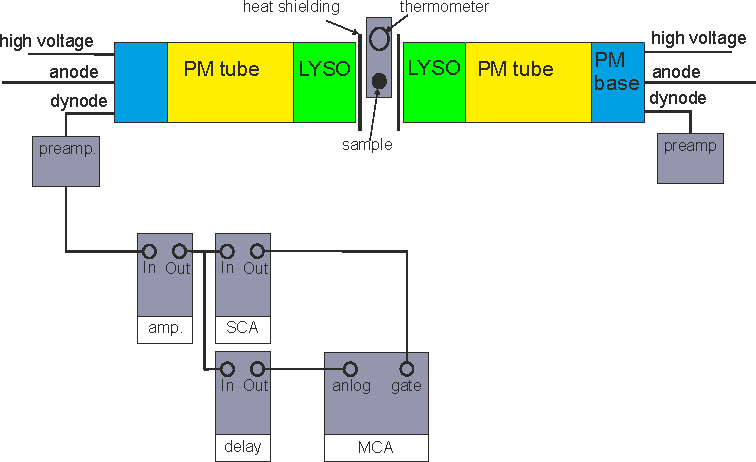
\includegraphics[width=0.8\textwidth]{./figures/aufbau/energie.pdf}
	\caption{Versuchsaufbau zur Einstellung des \textit{Slow}-Kreises und zur Aufnahme der Spektren \cite{anleitung}.}
	\label{fig:slow_kreis}
\end{figure}
In einem ersten Schritt muss die Verstärkung des \textit{Slow}-Kreises so eingestellt werden, dass die \SI{1275}{\keV}-Linie des angeregten Neon-Zustandes, welcher bei dem $\beta^+$-Zerfall von \isotope[22]{Na} entsteht, in den Spannungsbereich des MCA fällt.
Dies wird für jeden Detektor einzeln durchgeführt, indem parallel zu den SCAs ein \textit{Delay} eingesetzt wird, dessen Ausgang mit dem analogen Eingang des MCAs verbunden wird, während die SCAs das \textit{Gate}-Signal liefern.
Nachdem für beide Detektoren der Aufbau in Abbildung \ref{fig:slow_kreis} realisiert und die Koinzidenz von \textit{Slow}- und SCA-Signal verifiziert wurde, wird die \isotope[22]{Na}-Quelle in den Detektor eingeführt.
Zur Einstellung der Verstärkung wird die Fensterbreite des SCA maximiert und die untere Schwelle auf das Minimum gesetzt, sodass das gesamte Spektrum von Lutetium und Natrium bis zur~\SI{1275}{keV}-Linie (aus dem Natriumzerfall) noch beobachtbar ist.
Für den rechten Detektor war dies nicht vollständig möglich, da die maximale Fensterbreite des SCA nicht ausreicht um den gesamten Energiebereich von LYSO und Natrium abzudecken, obwohl der Verstärker auf minimale Verstärkung eingestellt wurde.
Daher wurde die untere Schwelle des SCA angehoben, bis die ~\SI{1275}{keV}-Linie durch den MCA aufgenommen werden konnte.

\subsection{Aufnahme von Energiespektren}
Nachdem die Verstärkung für beide Detektoren eingestellt wurde, wurde jeweils ein intrinsisches LYSO-Spektrum, sowie ein Spektrum mit der Natrium-Positronenquelle aufgenommen.
Diese wurden in den Abbildungen \ref{fig:lyso_spektren} und \ref{fig:na_spektren} dargestellt.
\begin{figure}[htbp]
	\centering
	\begin{subfigure}{\textwidth}
		\centering
		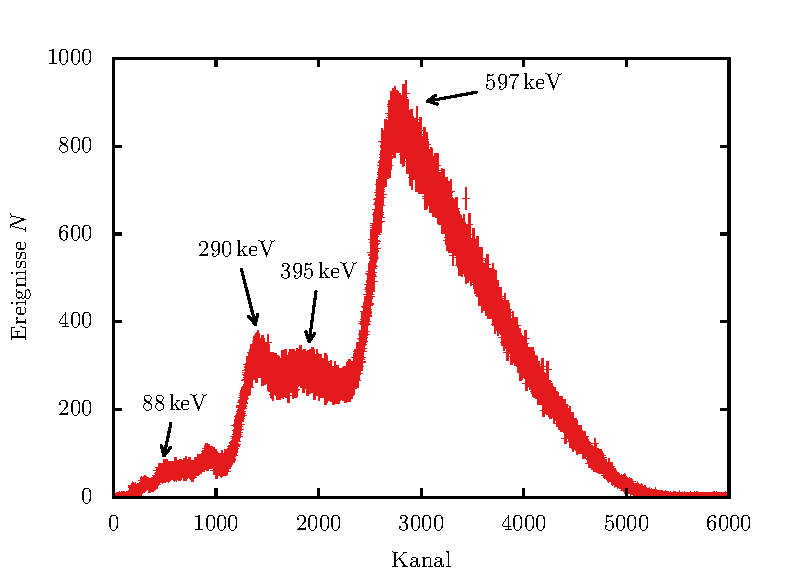
\includegraphics[width=\textwidth]{./figures/LYSO_links}
		\caption{LYSO Spektrum aufgenommen mit dem linken Detektor}
	\end{subfigure}
	\begin{subfigure}{\textwidth}
		\centering
		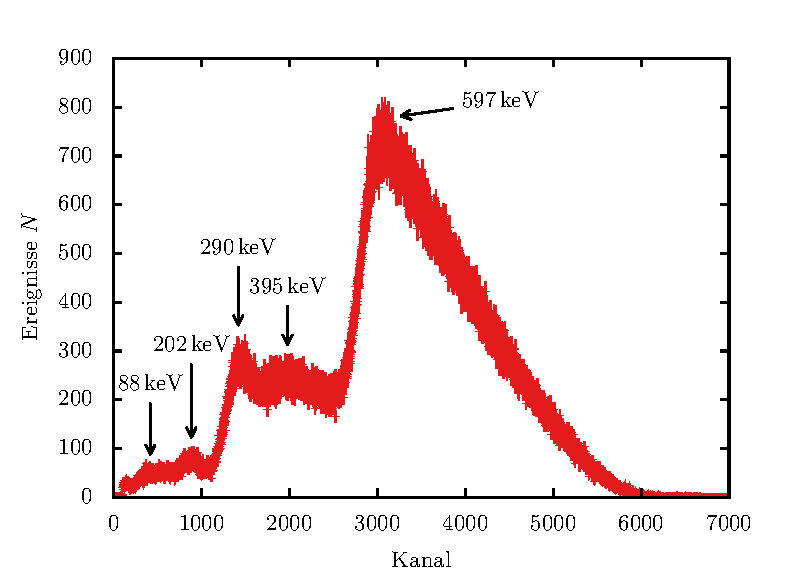
\includegraphics[width=\textwidth]{./figures/LYSO_rechts}
		\caption{LYSO Spektrum aufgenommen mit dem rechten Detektor}
	\end{subfigure}
	\caption{Spektren von Lutetium, das als Teil des Szintillatormaterials LYSO ein Gammaspektrum erzeugt. Die Maxima sind entsprechend der Photonenenergie gekennzeichnet.}
	\label{fig:lyso_spektren}
\end{figure}
\begin{figure}[htbp]
	\begin{subfigure}{\textwidth}
		\centering
		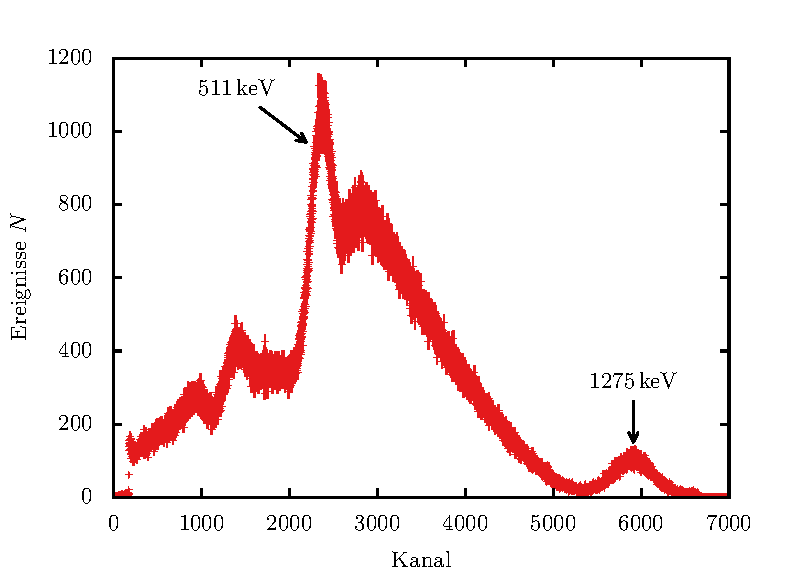
\includegraphics[width=\textwidth]{./figures/na_links}
		\caption{Spektrum von Natrium aufgenommen mit dem linken Detekor}
	\end{subfigure}
	\begin{subfigure}{\textwidth}
		\centering
		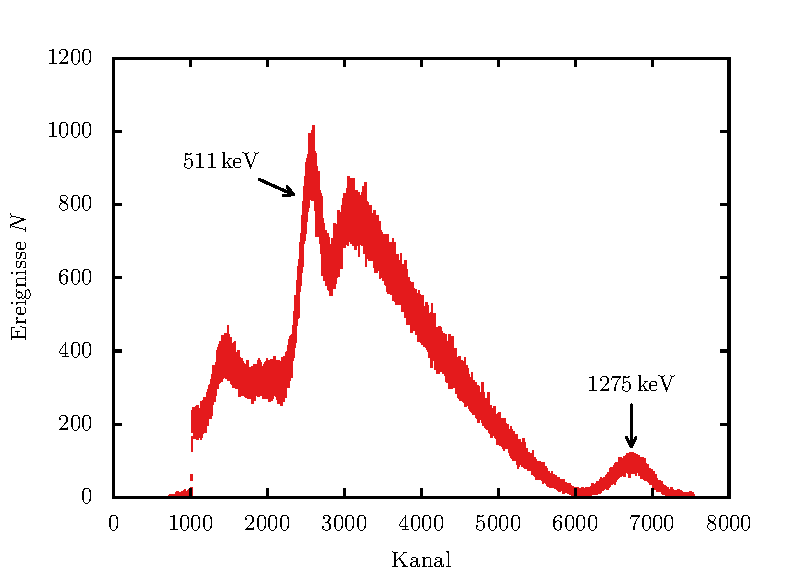
\includegraphics[width=\textwidth]{./figures/na_rechts}
		\caption{Spektrum von Natrium aufgenommen mit dem rechten Detekor}
	\end{subfigure}
	\caption{Spektren von Natrium. Es ist gut sichtbar, dass das Fenster des rechten SCAs zu klein ist, um bei minimaler Verstärkung das gesamte Spektrum aufzunehmen, weswegen ein deutlicher Schnitt bei Kanalnummer \num{1000} zu beobachten ist. Die Maxima des Untergrundes wurden nicht erneut gekennzeichnet, siehe hierfür Abb. \ref{fig:lyso_spektren}.}
	\label{fig:na_spektren}
\end{figure}
In den LYSO-Spektren können deutlich mehrere charakteristische Linien des radioaktiven Detektormaterials identifiziert werden.
Gemäß Abbildung~\korr{LUTETIUM-ZERFALLSSCHEMA} entsteht bei dem $\beta$-Zerfall von \isotope[176]{Lu} ein angeregter Hafnium-Zustand, welcher schnell über eine $\gamma$-Kaskade in den Grundzustand zerfällt.
Dabei treten hauptsächlich Photonen mit Energien von \SI{88}{\keV}, \SI{202}{\keV} und \SI{307}{\keV} auf.
Als Folge dessen bilden sich die charakteristischen Energiespektren aus Abbildung \ref{fig:lyso_spektren}, bei denen unter anderem Linien bei den Energien der einzelnen Photonen sichtbar sind.
Darüber hinaus 





Im Anschluss wurden die SCAs auf die~\SI{511}{keV}~Linie eingestellt, da diese aufgrund der höheren Rate zur Zeitkalibration genutzt wurde.

\subsection{Einstellung des \textit{Fast}-Kreises}
\label{ssec:fastkreis}
Im nächsten Schritt werden die Schwellen der CFDs im \textit{Fast}-Kreis eingestellt.
Hierzu wird das Signal des \textit{Slow}-Kreises auf dem Oszilloskop beobachtet, während das Signal der CFDs zum Triggern verwendet wird.
Die Schwelle wurde nun so eingestellt, dass gerade keine Nulllinie mehr auftrat.
Ein Beispiel eines solchen beobachteten Signals ist in Abbildung \korr{REF} zu sehen.
\korr{Abbildung}
Da die zu messenden Lebenszeiten sehr kurz sind, muss das Stopsignal verzögert werden, um eine korrekte Zeitmessung zu ermöglichen.
Dies geschieht, indem ein \si{ns}-Delay zwischen CFD des rechten Detektors und Eingang für das Stopsignal am TAC geschaltet wird.
Die Zeitverzögerung wird unter Beobachtung der Signale am Oszilloskop auf~\SI{20}{ns} eingestellt, wobei die gleichen Kabel wie zur späteren Messung verwendet werden sollten, da in diesen Größenordnungen bereits die Laufzeit des Signals berücksichtigt werden muss.
Um die gewünschte Verzögerung zu erreichen wurde eine zusätzliche Verzögerung am \textit{Delay}-Modul von~\SI{17.5}{ns} eingestellt.
Die interne Verzögerung beträgt laut Aufdruck auf dem Geärt~\SI{1.5}{ns} und die Kabellängen unterschieden sich um geschätzte~\SI{30}{cm}, so dass die gewählten Einstellungen durch eine einfache Abschätzung als plausibel bewertet werden können.

\subsection{Zeitkalibration}
Da die Zeitmessung durch eine zusätzliche Verzögerung beeinflusst wird, muss zur Interpretation der gemessenen Zeiten eine Kalibration erstellt werden.
Nachdem sowohl die Signal der beides SCAs im \textit{Slow}-Kreis als auch die Signale der \textit{Coincidence}-Einheit und des TACs aam Oszilloskop auf zeitliche Koinzidenz überprüft wurden, kann eine Promptkurve erstellt werden.
Hierbei wird das Stopsignal zusätzlich zur in~\ref{ssec:fastkreis} gewählten Verzögerung schrittweise um jeweils weitere~\SI{4}{ns} verzögert und für jede Einstellung über~\SI{2}{min} das entstehende Spektrum aufgenommen, welches in Abbildung~\ref{fig:promptkurven} gezeigt ist.
\korr{Abbildung}
Da aus den beobachteten Maxima die Zeitauflösung des Aufbaus bestimmt werden kann, wird eine Messung über~\SI{20}{min} von der Kurve mit keiner zusätzlichen Verzögerung durchgeführt.
Durch Anpassung einer Gaussfunktion kann die Zeitauflösung aus der Breite~$\sigma$ der beobachteten Kurve zu 
\begin{align*}
\num{48.30+-0.16}
\end{align*}
bestimmt werden.
Die zugehörigen Daten und Anpassung sind in Abbildung~\ref{fig:promptkurve_einzeln} dargestellt.

\begin{figure}[h]
	\centering
	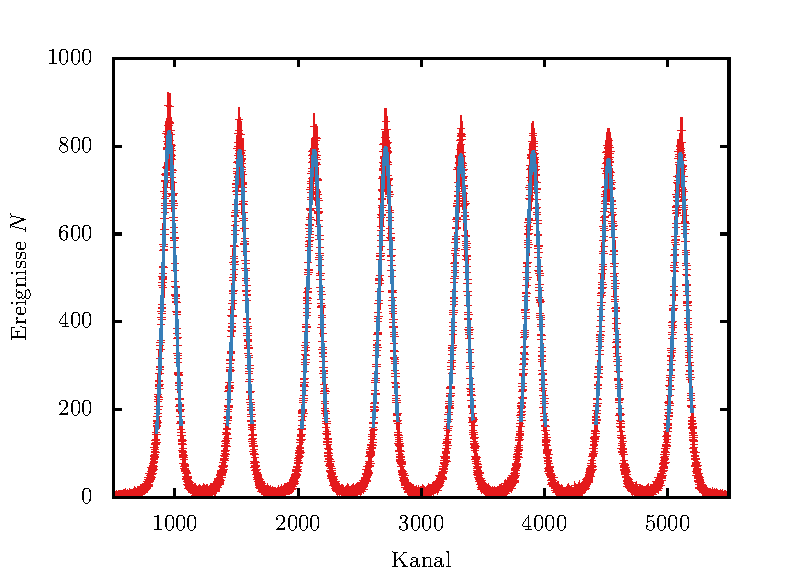
\includegraphics{./figures/prompt_curve_fits.pdf}
	\caption{Prompt-Kurven Fits}
	\label{fig:promptkurven}
\end{figure}

\begin{table}[h]
	\centering
	\begin{tabular}{SSS}
\toprule
{Verz�gerung~$\Delta t$ / \si{\nano\seconds}} & {Schwerpunkt~$\mu$ / Kanal} & {Schwerpunkt~$\sigma_\mu$ / Kanal} \\
\midrule
                                           20 &                      952.35 &                               0.20 \\
                                           24 &                     1525.73 &                               0.22 \\
                                           28 &                     2131.63 &                               0.22 \\
                                           32 &                     2711.83 &                               0.22 \\
                                           36 &                     3322.38 &                               0.22 \\
                                           40 &                     3908.53 &                               0.22 \\
                                           44 &                     4521.07 &                               0.22 \\
                                           48 &                     5105.48 &                               0.22 \\
\bottomrule
\end{tabular}

	\caption{Schwerpunkte des Fits}
\end{table}

\begin{figure}[h]
	\centering
	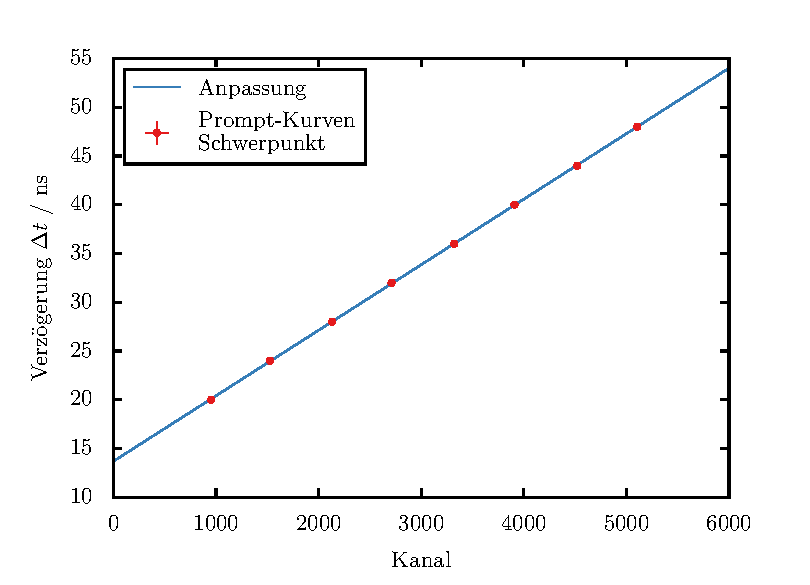
\includegraphics{./figures/prompt_curve.pdf}
	\caption{Zeitkalibrierung Prompt-Kurve}
\end{figure}


\begin{figure}[h]
	\centering
	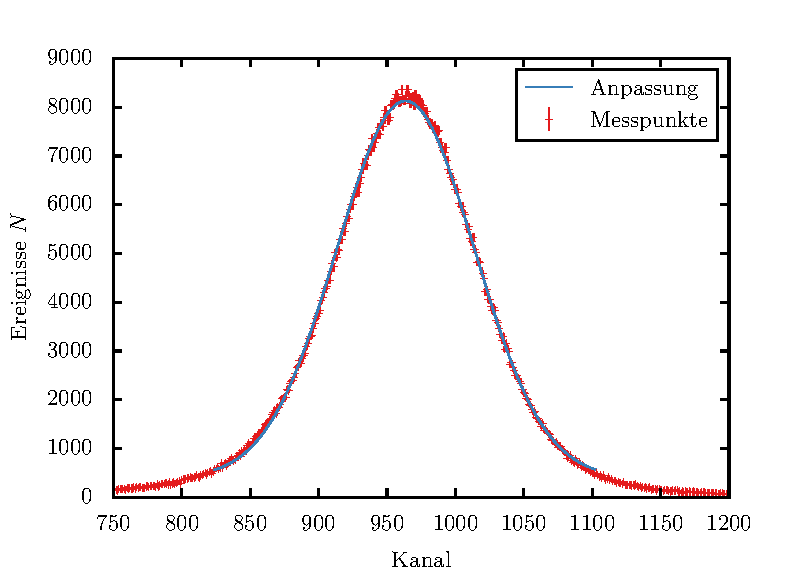
\includegraphics{./figures/fwhm_fit.pdf}
	\caption{FWHM Fit der Prompt Kurve}
	\label{fig:promptkurve_einzeln}
\end{figure}




\subsection{Messung der Lebensdauer mit Indium}

Nachdem die einzelnen Elemente des Messaufbaus überprüft und kalibriert wurden, werden die SCAs für die Messung der Lebensdauer eingestellt.
Da die beinahe gleichzeitig zur Positronenproduktion entstehenden Photonen als Startsignal genutzt werden, wird das Fenster des linken SCAs an die entsprechende Photonenenergie von~\SI{1275}{keV} angepasst.
Analog wird mit dem SCA für das Stopsignal, welches durch bei der Annihilation entstehende Photonen der Energie~\SI{511}{keV} entsteht, verfahren.
Danach kann mit der Messung der Lebensdauer begonnen werden.
Hierzu werden bei verschiedenen Temperaturen das vom TAC erzeugte Amplitudenspektrum gemessen.
Die Temperatur kann dabei über einen Lötkolben, der mit dem Probenhalter verbunden ist, geregelt werden.
Zur Temperaturmessung kommt ein digitales Thermometer zum Einsatz, dessen gemessene Werte durch ein zweites, analoges Thermometer im Temperaturbereich unter~\SI{100}{\degree\celsius} verifiziert werden konnten.
Als Messpunkt für die Temperatur wurde die mittlere Temperatur ausgehend von den Temperaturen zu Beginn und Ende der jeweiligen Messung verwendet.
Die Probe wurde so positioniert, dass eine Zählrate von ungefähr~\SI{60}{\per\second} erreicht wurde und die Software wurde auf eine Messdauer von genau~\SI{30}{min} eingestellt, so dass für jede Messung eine Statistik mit etwa~\num{100000} Einträgen entsteht.


\section{Lebenszeitmessung in Indium}

\section{Lebenszeitmessung in Acrylglas}

\section{Fazit}

\FloatBarrier
% BIBLIOGRAPHIE
\vspace{\fill}
% Maximale Anzahl der Einträge in Klammer
% Zitieren mit \cite{lamport94}
\begin{thebibliography}{19}
\bibitem{anleitung}
	\emph{Advanced Laboratory Course (physics601): Description of Experiments},
	BONN-AT-2016-01MP, Universität Bonn, Januar 2016.

\bibitem{wiki_standardmodell}
	\emph{Wikimedia Commons, the free media repository}. \url{https://commons.wikimedia.org/wiki/File:Standard_Model_of_Elementary_Particles-de.svg} (Letzter Aufruf: 15. März 2016)
	
\bibitem{script}
	N. Möser, J. Meier, J.-W. Tsung, E. von Törne,
	\emph{Der ATLAS-Versuch: Eigenschaften von W-Bosonen und die Suche nach neuer Physik}.
\bibitem{pdg}
	K.A. Olive \textit{et al.} (Particle Data Group),
	\emph{The Review of Particle Physics},
	Chin. Phys. C, \textbf{38}, 090001 (2014).

\bibitem{electron_atlas}
	ATLAS Collaboration (Aad, Georges \textit{et al.}),
	\emph{Electron performance measurements with the ATLAS detector using the 2010 LHC proton-proton collision data},
	Eur.\ Phys.\ J.\ C72 (2012) 1909.

\bibitem{odr}
	SciPy,
	\emph{Orthogonal distance regression (\texttt{scipy.odr})},
	\url{http://docs.scipy.org/doc/scipy/reference/odr.html} (Letzter Aufruf: 14. März 2016).

\bibitem{error_prop}
	B. Ochoa, S. Belongie,
	\emph{Covariance Propagation for Guided Matching},
	\url{http://vision.cornell.edu/se3/wp-content/uploads/2014/09/ochoa06.pdf} (Letzter Aufruf: 14. März 2016).
	
\bibitem{cern}
	CERN, \emph{Computer generated image of the whole ATLAS detector (CERN-GE-0803012-06)}, \url{http://cds.cern.ch/record/1095924} (Letzter Aufruf: 15. März 2016)
\end{thebibliography}

% APPENDIX
\begin{appendix}
\newpage
\section{Anhang}


\end{appendix}

\end{document}
